\documentclass[12pt,a4paper]{article}
\usepackage[utf8]{inputenc}
\usepackage[russian]{babel}
\usepackage{graphicx}
\usepackage{amsmath}
\usepackage{geometry}
\geometry{margin=2cm}
\usepackage{caption}
\usepackage{float}

\title{\\Сегментация и подсчет эритроцитов на изображениях мазков крови}
\author{Михайлова Анастасия Васильевна}

\begin{document}

\maketitle

\section*{Цель работы}

Изучить методы цифровой обработки изображений для автоматической сегментации и подсчета эритроцитов на микроскопических изображениях мазков крови.

\section*{Описание задачи}

В рамках работы требуется реализовать алгоритм, позволяющий автоматически выделять и подсчитывать эритроциты на изображениях мазков крови. Для этого используются методы фильтрации, выделения границ, морфологической обработки и анализа формы объектов.

\section*{Этапы обработки}

\begin{enumerate}
    \item \textbf{Исходное изображение} --- микроскопический снимок мазка крови.
    \item \textbf{Фильтрация и повышение контраста} --- медианная фильтрация, CLAHE.
    \item \textbf{Выделение границ} --- оператор Канни, Лапласиан.
    \item \textbf{Бинаризация и морфология} --- адаптивная пороговая обработка, морфологические операции.
    \item \textbf{Обнаружение эритроцитов} --- преобразование Хафа для кругов, уточнение контуров.
    \item \textbf{Визуализация результатов} --- наложение контуров и центров на исходное изображение.
\end{enumerate}

\section*{Используемые формулы}

\textbf{Медианная фильтрация:}
\begin{equation}
\operatorname{med}_{1 \leq k \leq N}\left[s_{k}\right]=
\begin{cases}
0.5(s_{n}+s_{n+1}), & N=2n \\
s_{n}, & N=2n-1
\end{cases}
\end{equation}
\noindent
Где $N$ --- размер окна, $s_k$ --- значения интенсивности в окне.

\textbf{Площадь круга:}
\begin{equation}
S = \pi r^2
\end{equation}
\noindent
$S$ --- площадь, $r$ --- радиус.

\textbf{Циркулярность:}
\begin{equation}
C = \frac{4\pi S}{P^2}
\end{equation}
\noindent
$C$ --- циркулярность, $S$ --- площадь, $P$ --- периметр.

\textbf{Преобразование Хафа для окружностей:}
\begin{equation}
(x - a)^2 + (y - b)^2 = r^2
\end{equation}
\noindent
$(a, b)$ --- координаты центра окружности, $r$ --- радиус.

\textbf{Градиент (для поиска границ):}
\begin{equation}
G = \sqrt{G_x^2 + G_y^2}
\end{equation}
\noindent
$G_x$, $G_y$ --- производные по $x$ и $y$.

\section*{Результаты}

\begin{figure}[H]
    \centering
    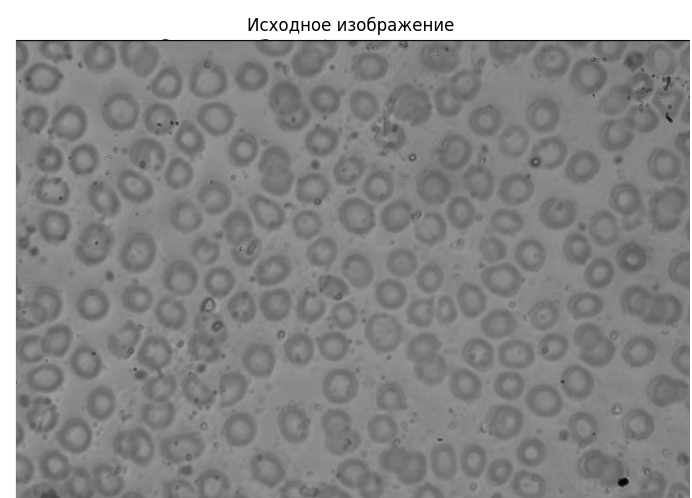
\includegraphics[width=0.45\textwidth]{original.png}
    \caption{Исходное изображение мазка крови}
\end{figure}

\begin{figure}[H]
    \centering
    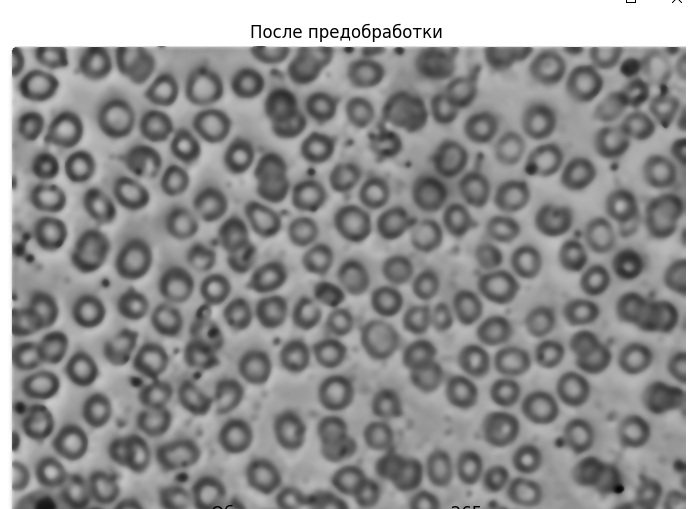
\includegraphics[width=0.45\textwidth]{preprocessed.png}
    \caption{После фильтрации и повышения контраста}
\end{figure}

\begin{figure}[H]
    \centering
    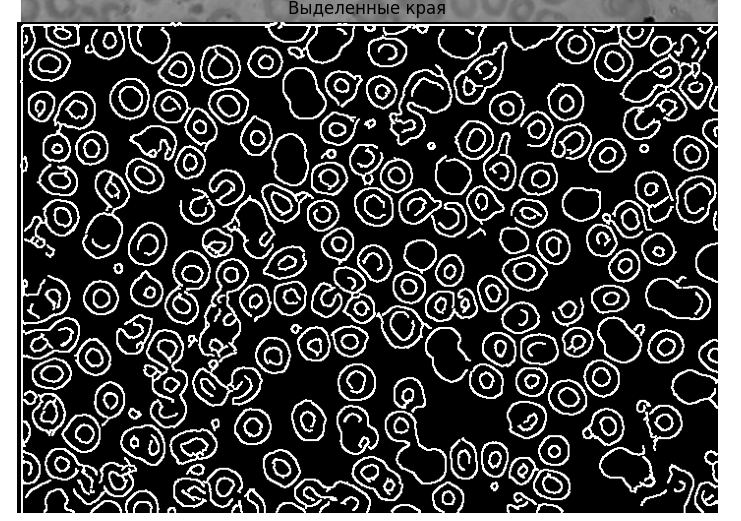
\includegraphics[width=0.45\textwidth]{edges.png}
    \caption{Выделенные границы}
\end{figure}

\begin{figure}[H]
    \centering
    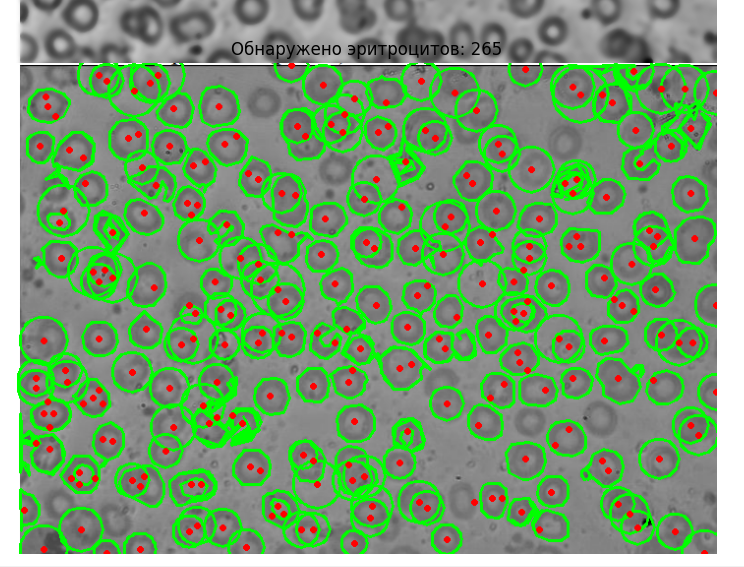
\includegraphics[width=0.45\textwidth]{result.png}
    \caption{Итог: обнаруженные эритроциты (контуры и центры)}
\end{figure}

\section*{Количественные результаты}

\begin{itemize}
    \item Обнаружено эритроцитов: \textbf{N}
    \item Точность/полнота (если есть ручная разметка): ...
\end{itemize}

\section*{Выводы}

В ходе работы был реализован и протестирован алгоритм автоматической сегментации и подсчета эритроцитов. Полученные результаты показывают высокую степень совпадения с визуальной оценкой, однако для 100\% точности требуется дополнительная ручная корректировка или использование методов машинного обучения.

\end{document} 